Based on the techniques and functionalities described in the previous
sections, we now show how to design and implement a subdivision
library for a generic CGAL polyhedron. This library is named
\emph{C}ombinatorial \emph{S}ubdivision
\emph{L}ibrary, short CSL. CSL contains a set of refinement 
functions and geometry smoothing rules that is user-customizable.
Subdivisions in CSL are specialized as a proper combination of the
refinement functions and the geometry smoothing rules.
%The goal of CSL are the 
%\emph{generic polyhedron data},
%\emph{user-friendly functional forms}, 
%\emph{user-customizable subdivisions}, and a
%\emph{extendible library}. 

CSL is designed based on the policy-based design 
\cite{Alexandrescu:2001:MCD}. The policy-based design assembles a class
(called \emph{host}) with complex behavior out of many small and
generic behaviors (called \emph{policies}).  Each policy defines an
\emph{interface} for a specific behavior and is customizable by the
user.  Policies are usually implemented as the functions or functors.
One gentle example is the \CodeFmt{for\_each} algorithm in STL
\footnote{\path|http://www.sgi.com/tech/stl/for_each.html|}. 
\begin{lstlisting}
template <class InputIterator, class UnaryFunction>
UnaryFunction for_each(InputIterator first, InputIterator last, UnaryFunction f);
\end{lstlisting}
The \CodeFmt{for\_each} is the algorithm host and the 
\CodeFmt{UnaryFunction f} is the generic behavior customizable 
by the user. To use it, user need to provide a policy functor
or function met the interface requirement of a unary function.

Based on the policy-based design, CSL
is designed to support both the \emph{generic types}, i.e.\ the polyhedron,
and the \emph{generic behaviors}, i.e.\ the subdivisions.
%This means users can customize the subdivisions at compile time. 
The interface of the generic types is specified as a \cgalpoly \ that
specifies both the connectivity and geometry interface.
The connectivity interface is required as primitive circulators or
the adjacency pointers of a halfedge. The geometry interface
is specified as \CodeFmt{Point} type of vertex items. The operational 
interface of the \CodeFmt{Point} is not specified by CSL and can 
be non-CGAL style. For non-CGAL \CodeFmt{Point}, users should
provide the user-defined policies that perform the point operations.

A subdivision algorithm has three key behaviors: \emph{refinement}, 
\emph{smoothing} and \emph{stencil correspondence}. The refinement is
acted as a \CodeFmt{for\_each} algorithm on the source \emph{and}
refined polyhedron while applying the smoothing behaviors. CSL
implement the refinements as the host functions with the smoothing
rules as the policies. Some major refinement schemes are shown in
\figurename\ \ref{fig:RefSchemes}. The accompanying CSL only
provides PQQ, PTQ and DQQ schemes. The refinements also define the
stencil correspondences; PQQ and DQQ cases are shown in 
\figurename\ \ref{fig:RefMap}. These stencil correspondences 
specified the functional interface between the refinement hosts 
and the geometry smoothing policies.

%% \cgalpoly\ provides two
%% mechanisms to implement refinements as introduced in the previous
%% sections. The geometry smoothing is mixed with the refinement
%% in the previous examples and hence implicitly maintain
%% the stencil correspondence. CSL extracts the geometry smoothing
%% from the refinement as policies and maintain the stencil 
%% correspondence explicitly. 


%-----------------------------------------------------------------------
\subsubsection{Primal Quad Quadralization}

\begin{figure}[htb]
    \centering{\includegraphics[width=12.0cm]{figs/TriCube_CC.eps}}
    \caption{Catmull-Clark subdivision of the box polyhedron.}
    \label{fig:cc}
\end{figure}

A subdivision algorithm in CSL is constructed as a
\emph{refinement function} parameterized with a set of the  
\emph{geometry smoothing rules}. The rule set is specified as
a template policy class. For example, Catmull-Clark
subdivision in CSL is instantiated as the PQQ scheme 
parameterized with a Catmull-Clark geometry policy class.
\begin{lstlisting}
void CatmullClark_subdivision(Polyhedron& p, int step = 1) {
  quad_quadralize_polyhedron(p, CatmullClark_rule<Polyhedron>(), step);
}
\end{lstlisting}
The \CodeFmt{quad\_quadralize\_polyhedron} is the refinement host
that refines the control polyhedron using PQQ scheme and the  
\CodeFmt{CatmullClark\_rule} is the template geometry policy class.
\\
%The refinement host applies the smoothing stencils provided by the 
%geometry policy class.

\noindent \textbf{Geometry policies} are represented as
the policy functions of the policy class. Each policy function
receive a \emph{primitive handle} of the represented 1-ring submesh 
of the control polyhedron; and a reference of the smoothing point
on the refined polyhedron. The interface of a policy class for a PQQ
refinement host is shown below.
\begin{lstlisting}
template <class _Poly>
class quadralize_rule {
public:
  void face_point_rule(Facet_handle, Point&) {};
  void edge_point_rule(Halfedge_handle, Point&) {};
  void vertex_point_rule(Vertex_handle, Point&) {};
};
\end{lstlisting}
The interface is defined according to the stencil correspondence of
the refinement scheme.  The PQQ scheme contains three stencils as
shown in
\figurename\ \ref{fig:RefMap} (a--c). Each of them
defines a policy function, which of the \CodeFmt{quadralize\_rule} 
is the \CodeFmt{facet\_rule()}, 
the \CodeFmt{edge\_rule()}, and the \CodeFmt{vertex\_rule()} 
respectively. Any customized policy class of the geometry 
smoothing rules are required to provide the proper functions.
To assure the interface consistence, CSL provides
a geometry rule class for each refinement scheme. To create a new
geometry policy class, the class inheritance is used.
\begin{lstlisting}
// Specialized a Catmull-Clark rule by inheriting the quadralize_rule.
template <class _Poly>
class CatmullClark_rule : public quadralize_rule<_Poly> {...}
\end{lstlisting}

The smoothing points of a refined polyhedron is generated by calling
the corresponding geometry policies.  Inside each policy, applying the
stencil is simplified into the mesh traversal of a 1-ring
neighborhood. It can be done with a primitive circulator or a simple
sequence of the adjacency pointers of the halfedges. The
\CodeFmt{face\_point\_rule} for Catmull-Clark subdivision demonstrates
the usage of a facet circulator for stenciling.
\begin{lstlisting}
  void face_point_rule(Facet_handle facet, Point& pt) {
    // Facet circulator is used to traverse the 1-ring of a facet.
    Halfedge_around_facet_circulator hcir = facet->facet_begin();
    int n = 0;
    Kernel::FT p[] = {0,0,0};
    // Apply the stencil while circulating around the facet. 
    do {
      Point t = hcir->vertex()->point();
      p[0] += t[0], p[1] += t[1], p[2] += t[2]; 
      ++n;
    } while (++hcir != facet->facet_begin());
    // Assign the smoothing point.
    pt = Point(p[0]/n, p[1]/n, p[2]/n);
  }
\end{lstlisting}
The facet circulator provides a convenient way to
traverse and collect the points. The point calculation use
the conventional interface \CodeFmt{[i]} of the point type. 
For \CodeFmt{Point} not equipped with the index access 
\CodeFmt{[i]}, a user-implemented policy class need to be 
provided. Though it should be an easy task as the example policy
shown. The CGAL \CodeFmt{Point\_3}/\CodeFmt{Vector\_3}
computation can be used if the \CodeFmt{Point} is the equivalent
type of \CodeFmt{Point\_3} which is shown below. 
\begin{lstlisting}
  void face_point_rule(Facet_handle facet, Point& pt) {
    Halfedge_around_facet_circulator hcir = facet->facet_begin();
    // Use CGAL::ORIGIN to transform Point into Vector.
    Vector vec = hcir->vertex()->point() - CGAL::ORIGIN;
    ++hcir;
    do {
      // Vector is a computational class
      vec = vec + hcir->vertex()->point();
    } while (++hcir != facet->facet_begin());
    // Use CGAL::ORIGIN to transform Vector back to Point.
    pt = CGAL::ORIGIN + vec/circulator_size(hcir);
  }
\end{lstlisting}

Instead of the circulator, the \CodeFmt{edge\_point\_rule} 
for Catmull-Clark subdivision requires the low lever 
halfedge traversal. It is simply done with the adjacency 
pointers of the halfedge item, i.e.\ the \CodeFmt{next()},
the \CodeFmt{prev()}, and the \CodeFmt{oppposite()}.
\begin{lstlisting}
  void edge_point_rule(Halfedge_handle edge, Point& pt) {
    Point p1 = edge->vertex()->point();
    Point p2 = edge->opposite()->vertex()->point();
    Point f1, f2;
    face_point_rule(edge->facet(), f1);
    face_point_rule(edge->opposite()->facet(), f2);
    pt = Point((p1[0]+p2[0]+f1[0]+f2[0])/4,
	       (p1[1]+p2[1]+f1[1]+f2[1])/4,
	       (p1[2]+p2[2]+f1[2]+f2[2])/4 );
  }
\end{lstlisting}
The \CodeFmt{edge->opposite()} is used to locate the opposite point
and the opposite facet. Instead of using the facet circulator for each
facet after obtaining the facet handle, the
\CodeFmt{face\_point\_rule} is called to calculate the facet
centroids. The smoothing point is then assigned as the centroid of the
two opposite points and the two facet centroids.

The \CodeFmt{vertex\_point\_rule} for Catmull-Clark subdivision
is more complicated than the other two policy functions. Unlike
the facet and edge rules, vertex rule is not static in the scenes
of the stencil weights. The weights are functions of the vertex 
valence and it introduces more geometry computations. 
Nonetheless, the connectivity traversal is still homomorphic to
a vertex circulation.  
\begin{lstlisting}
  void vertex_point_rule(Vertex_handle vertex, Point& pt) {
    // Only a vertex circulator is needed to collect the submesh.
    Halfedge_around_vertex_circulator vcir = vertex->vertex_begin();
    // The vertex valence is used to calculate the stencil weights.
    int n = circulator_size(vcir);

    float Q[] = {0.0, 0.0, 0.0}, R[] = {0.0, 0.0, 0.0};
    Point& S = vertex->point(); // The center vertex
    
    Point q;
    for (int i = 0; i < n; i++, ++vcir) {
      Point& p2 = vcir->opposite()->vertex()->point();
      R[0] += (S[0]+p2[0])/2; R[1] += (S[1]+p2[1])/2; R[2] += (S[2]+p2[2])/2;
      face_point_rule(vcir->facet(), q);
      Q[0] += q[0]; Q[1] += q[1]; Q[2] += q[2];
    }
    R[0] /= n;    R[1] /= n;    R[2] /= n;
    Q[0] /= n;    Q[1] /= n;    Q[2] /= n;
      
    // Assign the smoothing point.
    pt = Point((Q[0] + 2*R[0] + S[0]*(n-3))/n,
	       (Q[1] + 2*R[1] + S[1]*(n-3))/n,
	       (Q[2] + 2*R[2] + S[2]*(n-3))/n );
  }
\end{lstlisting}
Most of the codes are to do the geometry computations. The connectivity
operation is still a simple circulation.
\\

\noindent \textbf{Connectivity refinement} in CSL is 
design as a host function. A refinement host refines the input 
control polyhedron, maintains the stencil correspondence 
and assign the smoothed points. 
The \CodeFmt{quad\_quadralize\_polyhedron} is the refinement host
for a PQQ scheme. It redirects the refinement by 
repeating the \CodeFmt{quad\_quadralize\_1step()} that does 
one-step polyhedron refinement.
\begin{lstlisting}
// RULE is a template parameter specifying the geometry stencils. 
template <template <typename> class RULE>
void quad_quadralize_polyhedron(Polyhedron& p, RULE<Polyhedron> rule, int d) {
  // Do d times refinement.
  for (int i = 0; i < d; i++) quad_quadralize_1step(p, rule);
}
\end{lstlisting}
The \CodeFmt{quad\_quadralize\_1step()} is implemented
based on a sequence of the Euler operations which 
incrementally modify the connectivity.
\figurename\ \ref{fig:CCRefinement} illustrates the
incremental modifications for a PQQ scheme. 
\begin{lstlisting}
  // Build the connectivity using insert_vertex() and insert_edge()

  // Step1. Insert edge-vertices on all edges and set them to new positions.
  for (int i = 0; i < num_edge; i++, ++eitr) {
    Vertex_handle vh = insert_vertex(p, eitr);
    vh->point() = edge_point_buffer[i]; // Points are obtained with the edge rule.
  }
  fitr = p.facets_begin();
  for (int i = 0; i < num_facet; i++, ++fitr) {
    Halfedge_around_facet_circulator hcir_begin = fitr->facet_begin();
    Halfedge_around_facet_circulator hcir = hcir_begin;
    
    // Step2. Insert a cut-edge between 2 randomly selected incident edge-vertices.
    Halfedge_handle e1 = ++hcir;
    ++hcir; 
    Halfedge_handle e2 = ++hcir;
    ++hcir; // Must move the cir before inserts the new edge !!
    Halfedge_handle newe = insert_edge(p, e1, e2);
    
    // Step3. Insert a facet-vertex on the cut-edge and set it to the new position
    Halfedge_handle newv = insert_vertex_return_edge(p, newe);
    newv = newv->opposite()->prev(); // change newv to the larger face and 
                                     // still points to the newly inserted 
                                     // vertex
    // Update the geometry data of the face-vertex
    newv->vertex()->point() = face_point_buffer[i]; // Points are obtained with the facet rule.
   
    // Step4. Insert the facet-edges between the edge-vertices and the facet-vertex.
    while (hcir != hcir_begin) {
      e1 = ++hcir;
      ++hcir; // Must move the cir before inserts the new edge !!
      insert_edge(p, e1, newv); 
    }
  }
  // Update the geometry data of the vertex-vertices
  vitr = p.vertices_begin();
  for (int i = 0; i < num_vertex; i++, ++vitr) 
    vitr->point() = vertex_point_buffer[i]; // Points are obtained with the vertex rule.
\end{lstlisting}
The details of the Step2 and Step3 are shown in 
\figurename\ \ref{fig:CCRefinementStep23}. Note that the
\CodeFmt{insert\_vertex()} and \CodeFmt{insert\_edge()} are simple
connectivity functions composed of the Euler operators provided 
by \cgalpoly . Details about these two functions, readers should refer
to the \emph{lib\/SurfLab\/Polyhedron\_decorator.h}.
\\

\begin{figure}
  \centering 
  \psfrag{A}[]{Step1}
  \psfrag{B}[]{Step2}
  \psfrag{C}[]{Step3}
  \psfrag{D}[]{Step4}
  \epsfig{file=figs/CCRefinement.eps, width=10cm}
  \caption{A PQQ refinement of a facet is encoded into a sequence of
  vertex insertions and edge insertions. Red indicates the inserted
  vertices and edges in each step.}
  \label{fig:CCRefinement}
  \vspace{0.6cm}
  \epsfig{file=figs/CCRefinementStep23.eps, width=10cm}
  \caption{The Euler operations for the Step2 and Step3 of 
  the PQQ refinement.}
  \label{fig:CCRefinementStep23}
\end{figure}

\noindent \textbf{Stencil correspondence} is another key
behavior for a subdivision algorithm.
CSL refinement hosts employ the geometry policies
to generate the smoothing points. These points are then assigned 
to the corresponding refined vertices. Three temporary
point buffers, \CodeFmt{vertex\_point\_buffer}, 
\CodeFmt{edge\_point\_buffer} and \CodeFmt{face\_point\_buffer}, 
are used in the refinement host to store the points generated
by the geometry policies. Since CSL is designed
to accept a generic \cgalpoly , item flags in the 
Quad-Triangle example (described in the previous section) 
is not a feasible option for CSL. To maintain the stencil 
correspondence, CSL implicitly matches the storage 
order and operation order. The operation order is the
order of creating the vertices through the connectivity
operation in the refinement host. This order is demonstrated
in the \figurename\ \ref{fig:CCRefinement} and the related 
source code. Note \cgalpoly\ allocates new
geometry items by appending them at the end of the underlying
containers, in most cases the linked-list or the vector.
So the operation order is equivalent to the storage of the 
vertex items, hence the storage order of the points.
The storage order of the points is the also the order of calling 
the geometry policies.
CSL arranges the calling order of the geometry policies
to meet the operation order, which ensures the 
correspondence between the stencils and the points.
The smoothed points are generated 
from the geometry policies and stored in the temporary 
point buffers before assigned to the refined vertices.
\begin{lstlisting}
  // Build a new vertices buffer has the following structure:
  // 0 1 ... e_begin ... f_begin ... (end_of_buffer)
  // 0 ... e_begin-1       : store the points of the vertex-vertices
  // e_begin ... f_begin-1 : store the points of the edge-vertices
  // f_begin ... (end)     : store the points of the face-vertices
  int num_vertex = p.size_of_vertices();
  int num_edge = p.size_of_halfedges()/2;
  int num_facet = p.size_of_facets();

  // If Polyhedron is using vector, we need to reserve the memory to prevent 
  // the CGAL_assertion. We assume p is a quad-polyhedron.
  // This function for polyhedron using list is VOID.
  p.reserve(num_vertex+num_edge+num_facet, 4*2*num_edge, 4*num_edge/2);

  // Allocate the temporary point buffers.
  Point* vertex_point_buffer = new Point[num_vertex + num_edge + num_facet];
  Point* edge_point_buffer = vertex_point_buffer + num_vertex;
  Point* face_point_buffer = edge_point_buffer + num_edge;

  std::vector<bool> v_onborder(num_vertex);

  // Generate the facet points in the operation order.
  Facet_iterator fitr = p.facets_begin();
  for (int i = 0; i < num_facet; i++, ++fitr)
    rule.face_point_rule(fitr, face_point_buffer[i]);

  int sb = p.size_of_border_edges();

  // Generate the edge points in the operation order.
  Edge_iterator eitr = p.edges_begin();
  for (int i = 0; i < num_edge-sb; i++, ++eitr)
    rule.edge_point_rule(eitr, edge_point_buffer[i]);
    
  // Take care border point as another geometry policy. 
  for (int i = num_edge-sb; i < num_edge; i++, ++eitr) {
    int v = std::distance(p.vertices_begin(), eitr->vertex());
    v_onborder[v] = true;
    rule.border_point_rule(eitr, edge_point_buffer[i], vertex_point_buffer[v]);
  }

  // Generate the vertex points in the operation order.
  Vertex_iterator vitr = p.vertices_begin();
  for (int i = 0; i < num_vertex; i++, ++vitr)
    if (!v_onborder[i]) rule.vertex_point_rule(vitr, vertex_point_buffer[i]);
\end{lstlisting}
A border point policy is introduced to support the boundary case.
Border points usually have special stencil that in general degenerated from
2-variable surface to 1-variable curve. The full list of the refinement 
host and the geometry policies 
(including \CodeFmt{border\_point\_rule()}) can be found in the 
accompanying source code.


%-----------------------------------------------------------------------
\subsubsection{Dual Quad Quadralization}

\begin{figure}[htb]
    \centering{\includegraphics[width=12.0cm]{figs/TriCube_DS.eps}}
    \caption{Doo-Sabin subdivision of the box polyhedron.}
    \label{fig:ds}
\end{figure}

Primal schemes, such as PQQ, PTQ and $\sqrt{3}$ refinement, reserve
the control polyhedron or control vertices.  These schemes can devise
a sequence of Euler operations to incrementally manipulate the
connectivity while maintaining the stencil correspondence.  Dual
schemes, such as DQQ refinement, exchange the vertex and facet in the
process. These schemes lost the control vertices and hence are hard to
devise incremental manipulations. The modifier callback mechanism
supported by \cgalpoly\ is then used to implement such refinement
schemes.

CSL represents Doo-Sabin subdivision as a DQQ refinement 
parameterized with Doo-Sabin smoothing rules.
\begin{lstlisting}
void DooSabin_subdivision(Polyhedron& p, int step = 1) {
  dualize_polyhedron(p, DooSabin_rule<Polyhedron>(), step);
}
\end{lstlisting}
The \CodeFmt{dualize\_polyhedron()} is the refinement host and the
\CodeFmt{DooSabin\_rule} is a policy class supporting 
Doo-Sabin stencils.
\\

\noindent The \textbf{geometry policy} of a DQQ scheme is shown in
\figurename\ \ref{fig:RefMap} (d). The stencil centers around
a corner (as a facet-vertex pair) and defines the interface 
of the geometry policy. Only one geometry policy, i.e.\ the corner 
point, is needed for DQQ refinement. 
\begin{lstlisting}
template <class _Poly>
class dualize_rule {
public:
  // The corner is pointed by a halfedge handle.
  void point_rule(Halfedge_handle edge, Point& pt) {};
};
\end{lstlisting}
The \CodeFmt{Halfedge\_handle edge} points to the 
corner centered in the stencil submesh; and the 
\CodeFmt{Point\& pt} refers to the smoothing point
of the refined polyhedron. The implementation of the
Doo-Sabin stencil is shown below.
\begin{lstlisting}
template <class _Poly>
class DooSabin_rule : public dualize_rule<_Poly> {
public:
  void point_rule(Halfedge_handle he, Point& pt) {
    // The Doo-Sabin rule is a function of the facet degree.
    int n =  CGAL::circulator_size(he->facet()->facet_begin());

    // CGAL Vector computation is used for simple coding.
    Vector cv(0,0,0), t;
    if (n == 4) { // Regular facet.
      cv = cv + (he->vertex()->point()-CGAL::ORIGIN)*9;
      cv = cv + (he->next()->vertex()->point()-CGAL::ORIGIN)*3;
      cv = cv + (he->next()->next()->vertex()->point()-CGAL::ORIGIN);
      cv = cv + (he->prev()->vertex()->point()-CGAL::ORIGIN)*3;
      cv = cv/16;
    } else { // Extraordinary facet.
      double a;
      for (int k = 0; k < n; ++k, he = he->next()) {
	if (k == 0) a = ((double)5/n) + 1;
	else a = (3+2*std::cos(2*k*3.141593/n))/n;
	cv = cv + (he->vertex()->point()-CGAL::ORIGIN)*a;
      }
      cv = cv/4;
    }
    // Assign the smoothing point.
    pt = CGAL::ORIGIN + cv;
  }
};
\end{lstlisting}
The \CodeFmt{next()} of the halfedges around the 
facet is the only connectivity functionality needed 
to support Doo-Sabin stencil. 
Instead of using the conventional interface \CodeFmt{[i]} 
of the point type, we demonstrate the CGAL 
\CodeFmt{Point\_3}/\CodeFmt{Vector\_3} computation that gives
more succinct codes. For non-CGAL point type, a user-defined 
policy is required. 
\\

\noindent \textbf{Connectivity refinement} is implemented
based on the modifier callback mechanism (MCM). In the 
demonstration of Quad-Triangle subdivision, MCM is used to devise 
customized Euler-like atomic operators. In CSL, MCM is used to 
\emph{rebuild} the refinement polyhedron based on 
a complete facet-vertex index list. This method is called \emph{wholesale} 
scheme in contrast to the \emph{incremental} scheme of Euler operations.
%The facet-vertex index list is constructed on the encoded order
%of the connectivity.
The refinement host of a DQQ scheme is represented as the
\CodeFmt{dualize\_polyhedron()} and it
redirects the refinement by repeating a one-step
refinement function \CodeFmt{dualize\_1step()}.
\begin{lstlisting}
template <template <typename> class RULE>
void dualize_polyhedron(Polyhedron& p, RULE<Polyhedron> rule, int d = 1) {
  for (int i = 0; i < d; ++i) dualize_1step(p, rule);
}
\end{lstlisting}
The \CodeFmt{dualize\_1step()} first constructs a facet-vertex list
that is similar to the format of the OFF file or the OpenGL vertex
array. A facet-vertex list contains two buffers: a point buffer and a
facet index buffer. The point buffer stores the smoothing points
generated by the geometry policy, i.e.\ the \CodeFmt{point\_rule()}.
The points are generated in the order of the halfedge iterator. Note
each halfedge points to a corner that is a vertex on the refined
polyhedron.  The facet index buffer contains a list of the vertex
indices which depict facet polygons of the refined polyhedron. The
vertex indices point to the storage position in the point
buffer. Since each facet of the refined polyhedron is mapped into a
geometry primitive, i.e.\ vertex, edge, and facet, of the source
polyhedron, the facet order is defined by (and equal to) the iterator
order of the primitives in a \cgalpoly .
\begin{lstlisting}
template <class _P> template <template <typename> class RULE>
void Polyhedron_subdivision<_P>::dualize_1step(_P& p, RULE<_P> rule) {
  int num_v = p.size_of_vertices();
  int num_e = p.size_of_halfedges()/2; // Number of edges.
  int num_f = p.size_of_facets();
  int num_facet = num_v + num_e + num_f;
  
  // Init the facet-vertex list for the refined polyhedron.
  Point* point_buffer = new Point[num_e*2];
  int** facet_buffer = new int*[num_facet];
  for (int i = 0; i < num_facet; ++i) facet_buffer[i] = NULL;

  // Build the point buffer in the order of the halfedge iterator.
  Halfedge_iterator he_itr = p.halfedges_begin(); 
  for (int i = 0; i < num_e*2; ++i, ++he_itr) {
    Halfedge_around_facet_circulator cir = he_itr->facet_begin();
    // Generate the point with the geometry policy.
    rule.point_rule(cir, point_buffer[i]);
  }

  he_itr = p.halfedges_begin(); // Used to calculate the vertex index.
  // The vertex index is the distance of the halfedge iterator to its begin iterator.
  
  // Build the facet_buffer. Each refined facet corresponds to a control primitive.
  // Construct the facet-facet.
  Facet_iterator fitr = p.facets_begin();  
  for (int i = 0; i < num_f; ++i, ++fitr) {
    Halfedge_around_facet_circulator  cir = fitr->facet_begin();
    int n =  CGAL::circulator_size(cir); // Can be an extraordinary facet.
    facet_buffer[i] = new int[n+1];
    facet_buffer[i][0] = n;
    for (int j = 1; j < n+1; ++j, ++cir)
      facet_buffer[i][j] = 
	std::distance(he_itr, Halfedge_handle(cir.operator->())); 
  }
  // Construct the edge-facet.
  Halfedge_iterator eitr = p.halfedges_begin();
  for (int i = num_f; i < num_f+num_e; ++i, ++eitr) {
    facet_buffer[i] = new int[4+1];
    facet_buffer[i][0] = 4;
    facet_buffer[i][1] = (i-num_f)*2;
    facet_buffer[i][2] = std::distance(he_itr, eitr->prev());    
    ++eitr;
    facet_buffer[i][3] = (i-num_f)*2+1; 
    facet_buffer[i][4] = std::distance(he_itr, eitr->prev());    
  }
  // Construct the vertex-facet.
  Vertex_iterator vitr = p.vertices_begin();
  for (int i = num_f+num_e; i < num_f+num_e+num_v; ++i, ++vitr) {
    Halfedge_around_vertex_circulator  cir = vitr->vertex_begin();
    int n =  CGAL::circulator_size(cir); // Can be an extraordinary vertex.
    facet_buffer[i] = new int[n+1];
    facet_buffer[i][0] = n;

    for (int j = 1; j < n+1; ++j, --cir)
      facet_buffer[i][j] = 
	std::distance(he_itr, Halfedge_handle(cir.operator->())); 
  }
  
  // Rebuild the refined polyhedron. 
  p.clear();
  Polyhedron_memory_builder<Polyhedron> pb(num_e*2, point_buffer, 
					   num_f+num_e+num_v, facet_buffer);
  p.delegate(pb);
  
  // release the buffer of the new level
  for (int i = 0; i < num_facet; ++i) delete[] facet_buffer[i];
  delete[] facet_buffer;
  delete[] point_buffer;
}
\end{lstlisting}
After the facet-vertex list is build, 
the refined polyhedron is rebuild from the list with the 
modifier and the incremental builder.
\begin{lstlisting}
  Point* p = (Point*) point_buffer;
  pb.begin_surface(num_point, num_facet); {
    for (int i = 0; i < num_point; ++i) pb.add_vertex(p[i]);	
    for (int i = 0; i < num_facet; ++i) {
      pb.begin_facet(); {
	for (int n = 0; n < facet_buffer[i][0]; ++n)
	  pb.add_vertex_to_facet(facet_buffer[i][n+1]);
      }
      pb.end_facet();
    }
  }
  pb.end_surface();
\end{lstlisting}
The \CodeFmt{pb} is an object of the 
\CodeFmt{CGAL::Polyhedron\_incremental\_builder\_3}.

%-----------------------------------------------------------------------
\subsubsection{CSL}
CSL's policy-based approach offers a convenient way to specialize a
subdivision with a template geometry policy class.  The accompanying
source code of CSL supports Catmull-Clark, Loop, and Doo-Sabin
geometry policies and hence the subdivisions.  Each of the subdivision
is constructed by a proper combination of the refinement host and the
subdivision rules.  A customized subdivision can easily created with a
user-customized policy class. For example, a linear subdivision with
PQQ configuration is parameterized with average geometry rules.
\begin{lstlisting}
template <class _Poly>
class average_rule : public quadralize_rule<_Poly> {
public:
  // Generate the facet centroid.
  void face_point_rule(Facet_handle facet, Point& pt) {
    Halfedge_around_facet_circulator hcir = facet->facet_begin();
    int n = 0;
    FT p[] = {0,0,0};
    do {
      Point t = hcir->vertex()->point();
      p[0] += t[0], p[1] += t[1], p[2] += t[2]; 
      ++n;
    } while (++hcir != facet->facet_begin());
    pt = Point(p[0]/n, p[1]/n, p[2]/n);
  }
  // Generate the edge midpoint.
  void edge_point_rule(Halfedge_handle edge, Point& pt) {
    Point p1 = edge->vertex()->point();
    Point p2 = edge->opposite()->vertex()->point();
    pt = Point((p1[0]+p2[0])/2, (p1[1]+p2[1])/2, (p1[2]+p2[2])/2);
  }
  // Return the vertex itself.
  void vertex_point_rule(Vertex_handle vertex, Point& pt) {
    pt = vertex->point();
  }
};
\end{lstlisting}
Following function call invokes our new and simple linear PQQ subdivision.
\begin{lstlisting}
  quad_quadralize_polyhedron(poly, average_rule<Polyhedron>(), step);
\end{lstlisting}

Though demonstrated with a specific enriched \poly\ in our polyhedron
viewer, CSL accepts any polyhedron mesh specialized from the \poly\
. The only geometry requirement is the \CodeFmt{Point} type defined in
the vertex item.  Subdivisions in CSL are build as proper combinations
of the refinement functions and the geometry policy classes (hence the
name \emph{Combinatory} SL). The proper combination is constrained by
the stencil correspondence and checked in the compiler time.

Current version of CSL only supports the geometry modification of the
vertex (hence only the isotrophic subdivision). Boundary can be easily
supported by introducing the boundary policy. But for anisotropic
subdivisions (e.g.\ Pixar's crease rules), data modifications of the
halfedge are required. It can be done by introducing halfedge policy,
though a much complex structure is needed in the refinement host.

